\documentclass[table,aspectratio=43]{beamer}
% For a 16:9 example, set aspectratio=169

\usetheme[institute,webfont]{tugraz2018}
\institutelogo{beamerthemetugraz/institute/IAIK}

\usepackage[utf8]{inputenc}
\usepackage[english]{babel}

%%%%%%%%%%%%%%%%%%%%%%%%%%%%%%%%%%%%%%%%%%%%%%%%%%%%%%%%%%%%%%%%%%%%%%%%%%%%
% --- Optional packages for scientific content ---
\usepackage{listings}    % Source code listings
\usepackage{pgfplots}    % Plots and diagrams
\usepackage{tabu}        % Coloured tables -- requires [table] option for beamer
\usepackage{fontawesome} % Useful icons (\faName)
\usepackage[style=alphabetic,backend=biber]{biblatex} % Bibliography
\addbibresource{\jobname.bib}                         % Bibliography
\usepackage{filecontents}

%%%%%%%%%%%%%%%%%%%%%%%%%%%%%%%%%%%%%%%%%%%%%%%%%%%%%%%%%%%%%%%%%%%%%%%%%%%%
% --- Presentation metadata ---
\title[]{Presentation Examples}
\author[Jane Doe]{\textbf{Jane Doe} \and Mary Sue \and Gary Stu}
\date{SomeConf 2018}
\institute{IAIK}
\instituteurl{www.tugraz.at}


\begin{document}

  %%%%%%%%%%%%%%%%%%%%%%%%%%%%%%%%%%%%%%%%%%%%%%%%%%%%%%%%%%%%%%%%%%%%%%%%%%%%
  \begin{frame}[plain]
    \maketitle
  \end{frame}

  \begin{frame}
    \tableofcontents
  \end{frame}

  %%%%%%%%%%%%%%%%%%%%%%%%%%%%%%%%%%%%%%%%%%%%%%%%%%%%%%%%%%%%%%%%%%%%%%%%%%%%
  \section{Theme variants}

  %%%%%%%%%%%%%%%%%%%%%%%%%%%%%%%%%%%%%%%%%%%%%%%%%%%%%%%%%%%%%%%%%%%%%%%%%%%%
  \switchtostandard
  \title[]{Standard Titlepage\\Minimal Titlepage}
  \begin{frame}[plain]
    \maketitle
  \end{frame}

  \switchtoinstitute
  \title[]{Institute Titlepage}
  \begin{frame}[plain]
    \maketitle
  \end{frame}

  %%%%%%%%%%%%%%%%%%%%%%%%%%%%%%%%%%%%%%%%%%%%%%%%%%%%%%%%%%%%%%%%%%%%%%%%%%%%
  \switchtostandard
  \begin{frame}{Standard style}
  \end{frame}
  \switchtoinstitute
  \begin{frame}{Institute style}
  \end{frame}
  \switchtominimal
  \begin{frame}{Minimal style}
  \end{frame}
  \switchtostandard

  %%%%%%%%%%%%%%%%%%%%%%%%%%%%%%%%%%%%%%%%%%%%%%%%%%%%%%%%%%%%%%%%%%%%%%%%%%%%
  \section{Text and colors}

  %%%%%%%%%%%%%%%%%%%%%%%%%%%%%%%%%%%%%%%%%%%%%%%%%%%%%%%%%%%%%%%%%%%%%%%%%%%%
  \begin{frame}{Color palette}
    \begin{columns}[t]
      \column{.25\textwidth}
      \begin{beamercolorbox}[colsep*=4pt]{tug}tug = main\end{beamercolorbox}
      \begin{beamercolorbox}[colsep*=4pt]{fore}fore\end{beamercolorbox}
      \begin{beamercolorbox}[colsep*=4pt]{back}back\end{beamercolorbox}
      \begin{beamercolorbox}[colsep*=4pt]{foot}foot\end{beamercolorbox}
      \begin{beamercolorbox}[colsep*=4pt]{dark}dark\end{beamercolorbox}
      \begin{beamercolorbox}[colsep*=4pt]{lite}lite\end{beamercolorbox}
      \begin{beamercolorbox}[colsep*=4pt]{head}head\end{beamercolorbox}
      \begin{beamercolorbox}[colsep*=4pt]{body}body\end{beamercolorbox}
      \column{.25\textwidth}
      \begin{beamercolorbox}[colsep*=4pt]{arch}arch\end{beamercolorbox}
      \begin{beamercolorbox}[colsep*=4pt]{bauw}bauw (bau)\end{beamercolorbox}
      \begin{beamercolorbox}[colsep*=4pt]{etec}etec (etit)\end{beamercolorbox}
      \begin{beamercolorbox}[colsep*=4pt]{mach}mach (mbww)\!\!\end{beamercolorbox}
      \begin{beamercolorbox}[colsep*=4pt]{chem}chem (tcvp)\end{beamercolorbox}
      \begin{beamercolorbox}[colsep*=4pt]{info}info (infbio)\end{beamercolorbox}
      \begin{beamercolorbox}[colsep*=4pt]{math}math (mpug)\end{beamercolorbox}
      \column{.25\textwidth}
      \begin{beamercolorbox}[colsep*=4pt]{colA}colA\end{beamercolorbox}
      \begin{beamercolorbox}[colsep*=4pt]{colB}colB\end{beamercolorbox}
      \begin{beamercolorbox}[colsep*=4pt]{colC}colC\end{beamercolorbox}
      \begin{beamercolorbox}[colsep*=4pt]{colD}colD\end{beamercolorbox}
      \begin{beamercolorbox}[colsep*=4pt]{colE}colE\end{beamercolorbox}
      \begin{beamercolorbox}[colsep*=4pt]{colF}colF\end{beamercolorbox}
      Also:
      \textcolor{tugblue}{tugblue},
      \textcolor{tugred}{tugred}, \dots
    \end{columns}
  \end{frame}

  %%%%%%%%%%%%%%%%%%%%%%%%%%%%%%%%%%%%%%%%%%%%%%%%%%%%%%%%%%%%%%%%%%%%%%%%%%%%
  \begin{frame}{Structured text}

    \textbf{bold}, \textit{italics}, \textrm{roman}, \texttt{typewriter}, \underline{underlined},
    \bigskip

    \emph{Emphasis} (itshape)
    \bigskip

    \alert{Alert},  $a + \alert{b} = c$ (tug)
    \bigskip

    \structure{Structure},  $a + \structure{b} = c$ (main)
    \bigskip

    \textcolor{colD}{Color},  $a + {\color{colD} b} = c$
    \bigskip

    \highlight{Highlight (main)}
    \highlight[lite]{Highlight (lite)}
    \bigskip

    \url{www.tugraz.at} (urlA, ttfamily)
  \end{frame}

  %%%%%%%%%%%%%%%%%%%%%%%%%%%%%%%%%%%%%%%%%%%%%%%%%%%%%%%%%%%%%%%%%%%%%%%%%%%%
  \begin{frame}[fragile]{Font sizes}
    \thefontsize[TINY]\TINY
    \thefontsize[Tiny]\Tiny
    \thefontsize[tiny]\tiny
    \thefontsize[scriptsize]\scriptsize
    \thefontsize[footnotesize]\footnotesize
    \thefontsize[small]\small
    \thefontsize[normalsize]\normalsize
    \thefontsize[large]\large
    \thefontsize[Large]\Large
    \thefontsize[LARGE]\LARGE
    \thefontsize[huge]\huge
    \thefontsize[Huge]\Huge
  \end{frame}

  %%%%%%%%%%%%%%%%%%%%%%%%%%%%%%%%%%%%%%%%%%%%%%%%%%%%%%%%%%%%%%%%%%%%%%%%%%%%
  \section{Structuring the frame}

  %%%%%%%%%%%%%%%%%%%%%%%%%%%%%%%%%%%%%%%%%%%%%%%%%%%%%%%%%%%%%%%%%%%%%%%%%%%%
  \begin{frame}{Lists -- Basic}
    \texttt{itemize}:
    \begin{itemize}
      \item Item level 1
            \begin{itemize}
              \item Item level 2
                    \begin{itemize}
                      \item Item level 3
                    \end{itemize}
            \end{itemize}
    \end{itemize}

    \texttt{enumerate}:
    \begin{enumerate}
      \item Item level 1
            \begin{enumerate}
              \item Item level 2
                    \begin{enumerate}
                      \item Item level 3
                    \end{enumerate}
            \end{enumerate}
    \end{enumerate}
  \end{frame}

  %%%%%%%%%%%%%%%%%%%%%%%%%%%%%%%%%%%%%%%%%%%%%%%%%%%%%%%%%%%%%%%%%%%%%%%%%%%%
  \begin{frame}{Lists -- Variations}
    \texttt{tugitemize} with tighter spacing:
    \begin{tugitemize}
      \item Item level 1
      \begin{tugitemize}
        \item Item level 2
        \begin{tugitemize}
          \item Item level 3
        \end{tugitemize}
      \end{tugitemize}
    \end{tugitemize}

    \texttt{boxenumerate}:
    \begin{boxenumerate}
      \item Item level 1
      \begin{boxenumerate}
        \item Item level 2
        \begin{boxenumerate}
          \item Item level 3
        \end{boxenumerate}
      \end{boxenumerate}
    \end{boxenumerate}
  \end{frame}

  %%%%%%%%%%%%%%%%%%%%%%%%%%%%%%%%%%%%%%%%%%%%%%%%%%%%%%%%%%%%%%%%%%%%%%%%%%%%
  \newcommand{\checkyes}{\textcolor{tuggreen}{\faCheckSquareO}}
  \newcommand{\checkno}{\textcolor{black}{\faSquareO\,}}
  % Check out https://ctan.org/pkg/fontawesome
  \begin{frame}[fragile]{Lists -- Custom Icons with package \texttt{fontawesome}}
    Checklist:
    \begin{itemize}
      \item[\checkyes] Item 1
      \item[\checkyes] Item 2
      \item[\checkno] Item 3
    \end{itemize}
    Advantages and Disadvantages:
    \begin{itemize}
      \item[\textcolor{tuggreen}{\faPlusCircle}] Advantage
      \item[\textcolor{tugred}{\faMinusCircle}]  Disadvantage
      \item[\textcolor{tugblue}{\faArrowCircleRight}] Conclusion
    \end{itemize}
  \end{frame}

  %%%%%%%%%%%%%%%%%%%%%%%%%%%%%%%%%%%%%%%%%%%%%%%%%%%%%%%%%%%%%%%%%%%%%%%%%%%%
  \begin{frame}{Blocks}
    %
    \begin{block}{Block}
      dark+lite
    \end{block}
    %
    \begin{alertblock}{Alert Block}
      tug+lite
    \end{alertblock}
    %
    \begin{exampleblock}{Example Block}
      colE+lite
    \end{exampleblock}
  \end{frame}

  %%%%%%%%%%%%%%%%%%%%%%%%%%%%%%%%%%%%%%%%%%%%%%%%%%%%%%%%%%%%%%%%%%%%%%%%%%%%
  \begin{frame}{Blocks -- Math}
    \begin{theorem}[Theorem or Definition name]
      Content
    \end{theorem}
    %
    %\begin{definition}[Definition name]
    %  Content
    %\end{definition}
    %
    \begin{example}[Example name]
      Content
    \end{example}
    %
    \begin{proof}[Proof name]
      Content
    \end{proof}
  \end{frame}

  %%%%%%%%%%%%%%%%%%%%%%%%%%%%%%%%%%%%%%%%%%%%%%%%%%%%%%%%%%%%%%%%%%%%%%%%%%%%
  \begin{frame}{Side-by-side content}
    \begin{columns}[onlytextwidth]
      \begin{column}{0.5\textwidth}
        \begin{itemize}
          \item Lorem ipsum dolor sit amet, consectetur
          \item adipisicing elit, sed do eiusmod tempor
          \item incididunt ut labore et dolore magna aliqua.
        \end{itemize}
      \end{column}
      \begin{column}{0.5\textwidth}
        \begin{center}
          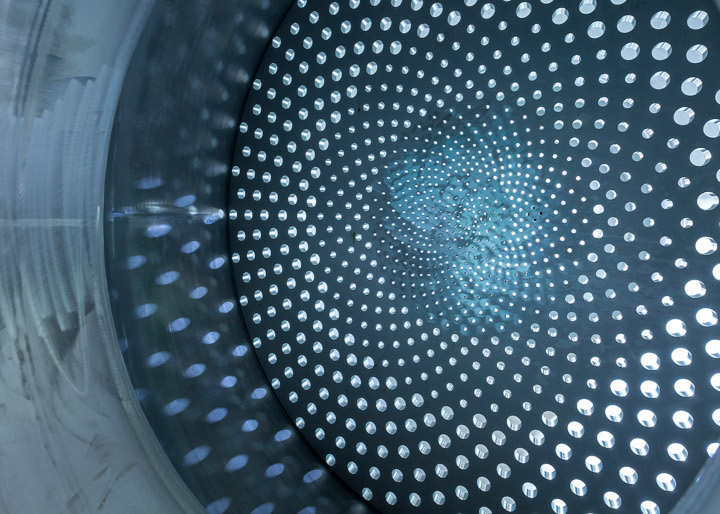
\includegraphics[width=0.75\textwidth]{figures/photoexample-43}\\
          A figure
        \end{center}
      \end{column}
    \end{columns}
  \end{frame}

  %%%%%%%%%%%%%%%%%%%%%%%%%%%%%%%%%%%%%%%%%%%%%%%%%%%%%%%%%%%%%%%%%%%%%%%%%%%%
  \begin{frame}[plain,c] % 'plain' hides theme elements
    \centering
    \Large Central standout text
  \end{frame}

  %%%%%%%%%%%%%%%%%%%%%%%%%%%%%%%%%%%%%%%%%%%%%%%%%%%%%%%%%%%%%%%%%%%%%%%%%%%%
  \fullscreenfigure{figures/photoexample-43}

  %%%%%%%%%%%%%%%%%%%%%%%%%%%%%%%%%%%%%%%%%%%%%%%%%%%%%%%%%%%%%%%%%%%%%%%%%%%%
  \section{Structuring the presentation}

  %%%%%%%%%%%%%%%%%%%%%%%%%%%%%%%%%%%%%%%%%%%%%%%%%%%%%%%%%%%%%%%%%%%%%%%%%%%%
  \begin{frame}{Outline}
    \tableofcontents[currentsection]
  \end{frame}

  %% Also try in the preamble:
  %\AtBeginSection[]
  %{
  %  \begin{frame}{Outline}
  %    \tableofcontents[currentsection]
  %  \end{frame}
  %}

  %%%%%%%%%%%%%%%%%%%%%%%%%%%%%%%%%%%%%%%%%%%%%%%%%%%%%%%%%%%%%%%%%%%%%%%%%%%%
  \sectionheader[Optional subtitle or figure]{Section Header}

  \sectionheader[\huge\color{tug}\faBalanceScale]{Section Header}

  %%%%%%%%%%%%%%%%%%%%%%%%%%%%%%%%%%%%%%%%%%%%%%%%%%%%%%%%%%%%%%%%%%%%%%%%%%%%
  \section{Technical content}

  %%%%%%%%%%%%%%%%%%%%%%%%%%%%%%%%%%%%%%%%%%%%%%%%%%%%%%%%%%%%%%%%%%%%%%%%%%%%
  \newcommand{\blue}[1]{{\color{tugblue}{#1}}}
  % Note that the standard CM fonts (the fallback for math symbols) are not scaled
  % correctly with the [webfont] and default [] options. If this bothers you, try
  %\usepackage{lmodern}
  %\usepackage[scale=1.1]{variablelm}
  \begin{frame}{Math and URLs}
    A multi-line equation about $\blue{x}$ and $\blue{t}$:
    \begin{align*}
      u(\blue{x},\blue{t}) & = \sum_{k=1}^{\infty} f_k \sin \frac{k \pi \blue{x}}{L} \cos \frac{k \pi \blue{t}}{aL} + \\
                           & + \sum_{k=1}^{\infty} g_k \sin \frac{k \pi \blue{x}}{L} \sin \frac{k \pi \blue{t}}{aL}
    \end{align*}
  \end{frame}

  %%%%%%%%%%%%%%%%%%%%%%%%%%%%%%%%%%%%%%%%%%%%%%%%%%%%%%%%%%%%%%%%%%%%%%%%%%%%
  \begin{frame}[fragile]{Verbatim}
    \begin{semiverbatim}
      Subject: Next meeting
      \alert{X-TUGAntiSpamFlag: spam}
      To: "Jane Doe" <jane.doe@tugraz.at>
      From: "Mary Sue" <mary.sue@tugraz.at>
    \end{semiverbatim}
  \end{frame}

  %%%%%%%%%%%%%%%%%%%%%%%%%%%%%%%%%%%%%%%%%%%%%%%%%%%%%%%%%%%%%%%%%%%%%%%%%%%%
  \begin{frame}[fragile]{Source code}
    \begin{lstlisting}[language=C,basicstyle=\ttfamily]
int find(int *A, int x, int n) {
  for(int i = 0; i < n; ++i) {
    if(A[i] == x) {
      return i;
    }
  }
  return -1;
}
  \end{lstlisting}
  \end{frame}

  %%%%%%%%%%%%%%%%%%%%%%%%%%%%%%%%%%%%%%%%%%%%%%%%%%%%%%%%%%%%%%%%%%%%%%%%%%%%
  \section{Tables and Diagrams}

  %%%%%%%%%%%%%%%%%%%%%%%%%%%%%%%%%%%%%%%%%%%%%%%%%%%%%%%%%%%%%%%%%%%%%%%%%%%%
  \begin{frame}{Table -- bold}
    % requires the tabu package
    \tabulinesep=2mm % wider spacing (default: 1mm)
    \begin{tabu}{lll}
      \tugtabu
      No.  & Title                           & Due \\
      D1.1 & Data Management Plan (DMP)      & M6  \\
      D1.2 & Intermediate Report             & M18 \\
      D1.3 & Final Report on Data Management & M36 \\
    \end{tabu}
  \end{frame}

  %%%%%%%%%%%%%%%%%%%%%%%%%%%%%%%%%%%%%%%%%%%%%%%%%%%%%%%%%%%%%%%%%%%%%%%%%%%%
  \begin{frame}{Table -- light}
    \begin{tabu}{lll}
      \tugtabulite
      No.  & Title                           & Due \\
      D1.1 & Data Management Plan (DMP)      & M6  \\
      \hline
      D1.2 & Intermediate Report             & M18 \\
      \hline
      D1.3 & Final Report on Data Management & M36 \\
      \hline
    \end{tabu}
  \end{frame}

  \begin{frame}{Table -- light}
    \footnotesize
    \begin{tabu}{X[L]X[L]X[L]}
      \tugtabulite
      Überschrift 1                    & Überschrift 2           & Überschrift 3    \\
      Platzhaltertext Information dazu & Das ist Platzhaltertext & Platzhaltertext  \\
      \hline
      Zweite Zeile                     & Und noch eine Zeile     & Mehr Information \\
      \hline
      Zweite Zeile                     & Und noch eine Zeile     & Mehr Information \\
      \hline
      Zweite Zeile                     & Und noch eine Zeile     & Mehr Information \\
      \hline
    \end{tabu}
  \end{frame}

  %%%%%%%%%%%%%%%%%%%%%%%%%%%%%%%%%%%%%%%%%%%%%%%%%%%%%%%%%%%%%%%%%%%%%%%%%%%%
  \begin{frame}{Color scheme for PGFplots}
    \centering
    \begin{tikzpicture}
      \begin{axis}[cycle list name=tug, no markers, every axis plot/.append style=thick,width=10cm,height=6cm]
        \addplot {rnd*.25-.25};
        \addplot {rnd*.25-0.5};
        \addplot {rnd*.25-0.75};
        \addplot {rnd*.25-1};
        \addplot {rnd*.25+x*0.05-0.75};
        \addplot {rnd*.25+x*0.05-0.75};
      \end{axis}
    \end{tikzpicture}
  \end{frame}

  %%%%%%%%%%%%%%%%%%%%%%%%%%%%%%%%%%%%%%%%%%%%%%%%%%%%%%%%%%%%%%%%%%%%%%%%%%%%
  \begin{frame}{Another Plot}
    \centering
    \begin{tikzpicture}
      \begin{axis}[ymin=0,ymax=1,enlargelimits=false,width=8cm,height=6cm]
        \addplot [colE,fill=colE,fill opacity=0.65,very thick] coordinates {
            (0,0.4) (0.2,0.75) (1,0.75)
          } |- (0,0) -- cycle;
        \addplot [colD,fill=colD,fill opacity=0.65,very thick] coordinates {
            (0,0.1)
            (0.1,0.15) (0.2,0.5)
            (0.3,0.62)
            (0.4,0.56) (0.5,0.58) (0.6,0.65) (0.7,0.6)
            (0.8,0.58) (0.9,0.55) (1,0.52)
          } |- (0,0) -- cycle;
        \addplot [colA,fill=colA,opacity=0.65,very thick] coordinates {
            (0,0.25)
            (0.1,0.27) (0.2,0.24) (0.3,0.24)
            (0.4,0.26) (0.5,0.3)
            (0.6,0.23) (0.7,0.2)
            (0.8,0.15) (0.9,0.1)
            (1,0.1)
          } |- (0,0) -- cycle;
      \end{axis}
    \end{tikzpicture}
  \end{frame}

  %%%%%%%%%%%%%%%%%%%%%%%%%%%%%%%%%%%%%%%%%%%%%%%%%%%%%%%%%%%%%%%%%%%%%%%%%%%%
  \begin{frame}{Bar Chart}
    \centering
    \begin{tikzpicture}
      \begin{axis}[
          %title={Diagram title},
          enlargelimits=0.15,
          font=\scriptsize,
          legend style={at={(0.5,-0.15)}, anchor=north,legend columns=-1,font=\scriptsize,draw=none},
          width=1.0\textwidth,height=.7\textheight,
          ybar,
          cycle list name=tugfill,
          bar width=5pt,
          ymajorgrids,
          symbolic x coords={Kategorie 1, Kategorie 2, Kategorie 3, Kategorie 4},
          xtick=data,
          xtick style={draw=none},xtick pos=left,xticklabel shift=-4pt,
          ymin=0,ymax=5.5,ytick distance=1,
          enlarge y limits=false,
        ]
        \addplot coordinates {
            (Kategorie 1,4.1)
            (Kategorie 2,2.5)
            (Kategorie 3,3.5)
            (Kategorie 4,4.5)
          };
        \addplot coordinates {
            (Kategorie 1,2.2)
            (Kategorie 2,4.5)
            (Kategorie 3,1.8)
            (Kategorie 4,2.8)
          };
        \addplot coordinates {
            (Kategorie 1,4.5)
            (Kategorie 2,3.5)
            (Kategorie 3,1.5)
            (Kategorie 4,2.5)
          };
        \addplot coordinates {
            (Kategorie 1,3.8)
            (Kategorie 2,2.8)
            (Kategorie 3,1.8)
            (Kategorie 4,4.8)
          };
        \addplot coordinates {
            (Kategorie 1,2.3)
            (Kategorie 2,3.3)
            (Kategorie 3,4.3)
            (Kategorie 4,1.3)
          };
        \addplot coordinates {
            (Kategorie 1,3.1)
            (Kategorie 2,2.1)
            (Kategorie 3,1.1)
            (Kategorie 4,4.1)
          };
        \legend{Reihe 1,
          Reihe 2,
          Reihe 3,
          Reihe 4,
          Reihe 5,
          Reihe 6}
      \end{axis}
    \end{tikzpicture}
  \end{frame}

  %%%%%%%%%%%%%%%%%%%%%%%%%%%%%%%%%%%%%%%%%%%%%%%%%%%%%%%%%%%%%%%%%%%%%%%%%%%%
  \begin{frame}{Pie Chart}
    \centering
    \begin{tikzpicture}[thick]
      \pgfmathsetmacro{\globalsumperc}{0}

      \foreach \name/\col/\perc in {A/colA/10,
          B/colB/20,
          C/colC/30,
          D/colD/9,
          E/colE/9,
          F/colF/22} {
          \pgfmathsetmacro{\sumperc}{\globalsumperc+\perc}
          \draw[white,fill=\col] (0,0) -- (\globalsumperc*3.6:2cm) arc [start angle=\globalsumperc*3.6, end angle=\sumperc*3.6, radius=2cm] -- cycle;
          \draw[white] (\globalsumperc*3.6+\perc*1.8:1.25cm) node {\perc\%};
          \global\let\globalsumperc=\sumperc
        }
    \end{tikzpicture}
  \end{frame}

  %%%%%%%%%%%%%%%%%%%%%%%%%%%%%%%%%%%%%%%%%%%%%%%%%%%%%%%%%%%%%%%%%%%%%%%%%%%%
  \section{Bibliography}

  %%%%%%%%%%%%%%%%%%%%%%%%%%%%%%%%%%%%%%%%%%%%%%%%%%%%%%%%%%%%%%%%%%%%%%%%%%%%
  \begin{frame}{Bibliographic references}
    Short citation: \cite{cryptoAuthor18}

    In their paper, \textcite{cryptoAuthor18} show that \dots % requires biblatex
  \end{frame}

  %%%%%%%%%%%%%%%%%%%%%%%%%%%%%%%%%%%%%%%%%%%%%%%%%%%%%%%%%%%%%%%%%%%%%%%%%%%%
  \begin{frame}[allowframebreaks]{Bibliography}
    \printbibliography
  \end{frame}

  %%%%%%%%%%%%%%%%%%%%%%%%%%%%%%%%%%%%%%%%%%%%%%%%%%%%%%%%%%%%%%%%%%%%%%%%%%%%
  \setbeamertemplate{bibliography item}[book]
  \begin{frame}[allowframebreaks]{Bibliography}
    \printbibliography
  \end{frame}

  \begin{filecontents*}{\jobname.bib}
    @inproceedings{cryptoAuthor18,
      author       = {First Author and
          Second Author and
          Third Author},
      title        = {On Publications and their Bibliographic Representation},
      booktitle    = {CONF 2018},
      publisher    = {Springer},
      year         = {2018},
    }
\end{filecontents*}

\end{document}
